\chapter{Paradigmes architecturaux des plateformes Multicœurs-UMA/NUMA}
%
Dans ce chapitre, 
nous introduisons les concepts concernant les supports matériels responsables de l'exécution des applications parallèles. 
L'objectif est de présenter les particularités techniques et les spécificités architecturales des différents types de plateformes parallèles.
Pour concevoir des ordonnanceurs efficaces qui puissent tirer parti efficacement (et si possible facilement) des architectures parallèles, 
il faut exploiter certaines caractéristi-ques liées à la spécificité du type ciblé. 
En effet, pour obtenir de bonnes performances, les applications parallèles doivent exploiter les avantages de l’architecture sous-jacente et les services proposés par le support exécutif (runtime). 
Les ordinateurs actuels disposent de plusieurs niveaux de parallélisme matériel. 
Ils peuvent disposer de plusieurs processeurs connectés par un réseau d'interconnexion, qui eux-mêmes sont composés de plusieurs cœurs, et ces cœurs disposent d’unités de calcul vectoriel. 

%2.1
Dans la section 2.1, 
nous décrivons tout d’abord les architectures des processeurs monocoeurs. 
Nous détaillerons les différentes limitations physiques qui régissent ces archite-ctures. 
%2.2
Puis, dans la section 2.2, 
nous considérons un autre type de plateforme qui sera le successeur du monoprocesseur, les multicœurs, nous nous intéressons à cette architecture et à ses caractéristiques.
%2.3
La section 2.3 expose le premier type des plateformes multiproce-sseurs UMA/SMP.
%2.4
La plateforme NUMA, qui sera l'objet de notre étude, est présentée dans la section 2.4.
%2.5
Enfin, la section 2.5 présente le problème du placement des données en introduisant le concept de la localité des données ainsi que la terminologie associée dans ce contexte.
%======================================================================================================
\section{Processeurs monocœur}
%
Depuis son invention en 1969 et sa première commercialisation en 1971, le \textbf{micro-processeur} a suivi une évolution phénoménale en doublant sa capacité de traitement tous les deux ans comme il a prédit le cofondateur d’Intel Mr \textbf{G. Moore} dans son article de 1965 que le nombre des transistors sur les puces semi-conducteurs va doubler chaque 18 mois. Ce nombre est déterminé par l’évolution de la \textbf{finesse de gravure} dont la diminution permet d'augmenter ce nombre par puce et aussi sa fréquence \cite{moor65}. Durant cette évolution, les processeurs ont connu une succession de transformation dans ses versions (single cycle processor, Pipelined , Deep-Pilepline, Superscalar, Out-of Order) \cite{qaca17}.

Jusqu’au début des années deux mille, Les performances des processeurs construits sur le \textbf{modèle de von Neumann} ont continué d’augmenter de façon exponentielle. Au cours des années, les processeurs sont devenus de plus en plus petits. Cette diminution affecte directement, en termes de fréquence, leurs performances. Ces dernières années, Cette augmentation amorce un fort ralentissement (Table \ref{table:TB_2_1} donne la tendance de l'augmentation de la puissance par date).

\begin{table}[h!]
\centering
\begin{tabular}{| c |c | c | c|} 
\hline
Année & 1990 & 2000 & 2004 \\ [0.5ex] \hline
Augmentation de puissance & 60\% & 40\% & 20\% \\ [1ex] 
\hline
\end{tabular}
\caption{Augmentation de la puissance de 1990 à 2004 \cite{qaca17}}
\label{table:TB_2_1}
\end{table}

Les contraintes qui ont freiné cette évolution sont exprimées par le terme "\textbf{Patter-son three walls}" [Berkeley's David Patterson succinctly summarized INTEL's problem in "Patterson's Three Walls": Power Wall + Memory Wall + ILP Wall = Brick Wall]\cite{russ10} qui désigne les barrières (murs) confrontés par les méthodes et les technologies utilisées dans le processus de fabrication des processeurs. Alors elles ont atteint leurs limites. Les trois mur/barrières de Patterson sont :
%
\subsection{Puissance}
%
La diminution de finesse de gravure a permis de mettre plus de transistors par la même puce qui ont besoin de plus de puissance qui va entrainer une consommation électrique et une dissipation thermique importantes. %En plus que 
Ce processus (finesse de gravure) a une limite physique que toute technologie utilisée pour cette opération est incapable d'aller au delà de cette limite. En effet, il se heurt à des phénomènes physiques limitant les performances. La table \ref{table:TB_2_2} donne la tendance de la finesse de gravure par date depuis 1978  jusqu'à 2015 et les prévisions pour l'année 2021 et 2028 (qui sera la fin du processus de la diminution de la taille physique de la grille des transistors à 5nm \cite{toms16}).

\begin{table}[h!]
\centering
\begin{tabular}{| c | c | c | c | c | c | c | c|} 
\hline
Année                  & 1978    & 1985  & 1995  & 2005  & 2015  & 2021  & 2028 \\ [0.5ex] \hline
Finesse de Gravure & 100nm & 52nm & 35nm & 25nm & 15nm & 10nm & 5nm \\ [1ex]  \hline
\end{tabular}
\caption{Finesse de la gravure de 1978 à 2028 src : \cite{toms16}} %
\label{table:TB_2_2}
\end{table}

Donc, l’augmentation de la \textbf{fréquence}, pour permettre celle des performances, a atteint ses limites. 
Ces dernières sont proportionnelles au produit du nombre de transistors par la \textbf{fréquence d’horloge}. 
En effet, un transistor consomme et dissipe à chaque changement d’état. 
Donc, plus il y a de transistors, plus il y a de consommation électrique et de dissipation thermique. 
Ce phénomène est amplifié par la fréquence d’horloge qui va augmenter la fréquence des changements d’état et donc la consommation et la dissipation. 
La consommation électrique et la dissipation thermique ont aujourd’hui atteint des seuils critiques avec certains processeurs ayant  une consommation de plus de 100W et nécessitant d’imposants systèmes de refroidissement.
Donc, Nous ne pouvons plus augmenter la fréquence des processeurs avec la conception actuelle des transistors. La figure \ref{fig:FG_2_1} donne l'évolution des fréquences maximales des processeurs durant ces derniers 40 ans.

\begin{figure}[h]
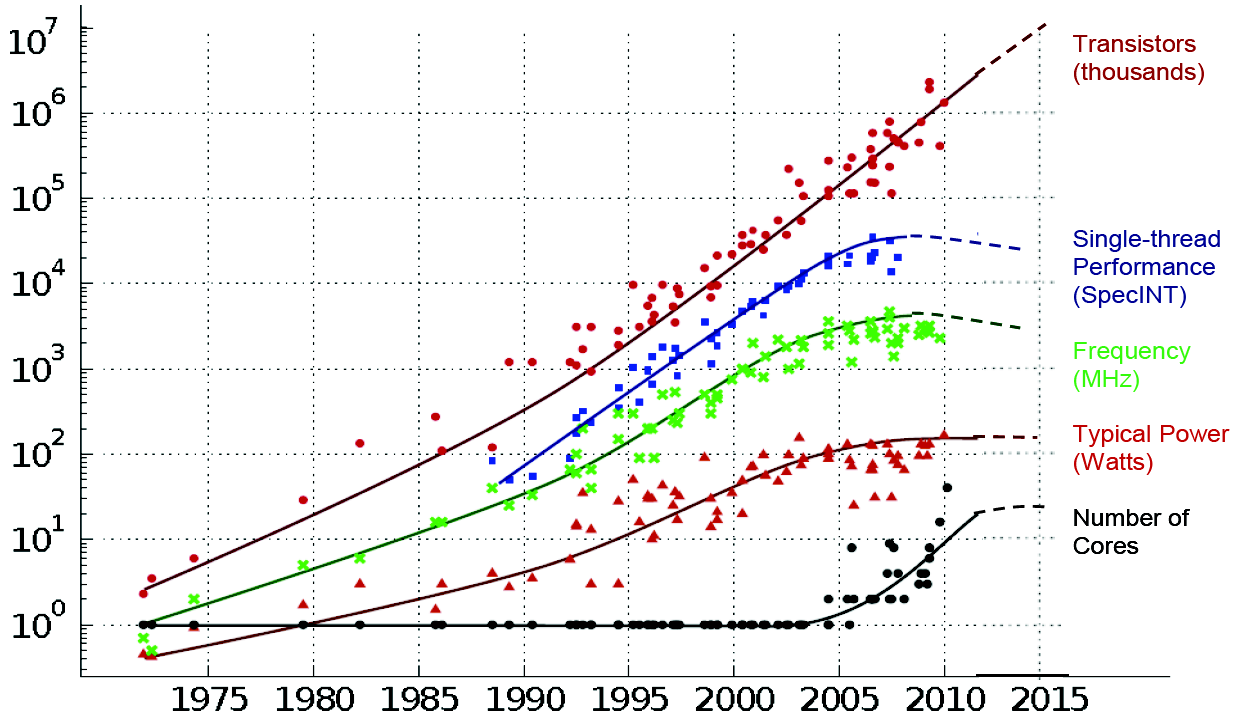
\includegraphics[scale=0.35]{cpu_trands}
\centering
\caption{Evolution des fréquences maximales de processeurs \cite{qaca17}}
\label{fig:FG_2_1}
\end{figure}
%
\subsection{Mémoire}
%
Une caractéristique importante du développement matériel au cours des dernières décennies a été l'écart croissant entre le \textbf{temps de cycle de l'horloge du processeur} et le \textbf{temps d'accès à la mémoire} principale. 
La mémoire principale est construite sur la base de la mémoire \textbf{DRAM (Dynamic Random Access Memory)} qui est trop lente par rapport au cycle d'horloge du CPU.
Les calculs impliquant uniquement le registre du processeur peuvent être effectués rapidement, mais lors d'un accès à la mémoire principale, le processeur se bloque pendant de nombreux cycles en attendant les données de la mémoire avant de pouvoir reprendre l'exécution et cela limite fortement ses performances. Durant cette opération, beaucoup de cycles sont perdus à attendre que des données en mémoire soient mises dans les registres.
Cet écart (de la vitesse entre le processeur et la mémoire) est devenu très grand ce qui rend inutile de continuer cette course qui n'est pas suivie par la mémoire.
En effet, la différence entre la fréquence du processeur et celle de la mémoire est telle que tout accès mémoire devient extrêmement coûteux (memory wall \cite{memw04}).
La figure \ref{fig:FG_2_2} donne l'écart de la vitesse entre le processeur et la mémoire.

\begin{figure}[h]
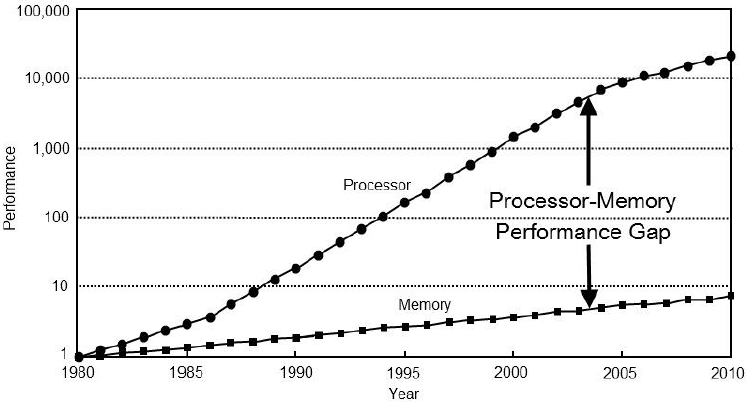
\includegraphics[scale=0.5]{ram_gap}
\centering
\caption{Ecart de la vitesse entre le processeur et la mémoire \cite{memw04}}
\label{fig:FG_2_2}
\end{figure}
%
\subsection{Pipeline ILP( Instruction Level Parallelism)}
%
Le \textbf{parallélisme matériel} a atteint sa limite de 40 étages au delà il y a peu de parallélisme avec un coût important (Extraction du parallélisme au niveau des instructions à partir d’un flot séquentiel bas niveau). 

"L'industrie a été stupéfaite lorsque Intel a annulé non pas un, mais deux modèles de processeurs de premier plan en mai 2004. Intel Tejas (le mono remplaçant de Pentium 4) a dissipé 150 watts à 2,8 GHz avec un pipeline de 40 étages et un socket 1000 pins. Lorsque les microprocesseurs sont trop chauds, ils cessent de fonctionner et parfois explosent." Suite à cet évènement, l'expression "Intel's Tejas hits the walls - hard" a exprimé la situation de l'industrie des microprocesseurs, en marquant la fin de la période des monoprocesseurs .
Ainsi, Intel a rapidement changé de direction, et a annoncé le premier double cœur processeur en lançant la révolution des multicœurs. \cite{russ11}
%======================================================================================================
\section{Processeurs Multicœurs (Multicore)}
%
Le \textbf{processeur multicœurs} est un processeur intégrant plusieurs unités de calcul en les dupliquant sur la même puce. 
On appelle chaque unité un \textbf{cœur (core)} qui est capable de faire un traitement, d'accéder à la mémoire, d'exécuter des entrées/sorties, qui est superscalaire, out-of-order et dispose d’un certain nombre d’unités de calcul vectoriel (Single Instruction Multiple Data ou SIMD). 
L'ensemble des cœurs fonctionne en parallèle en réalisant les tâches affectées (calcule, communication RAM - I/O).

\begin{figure}[h]
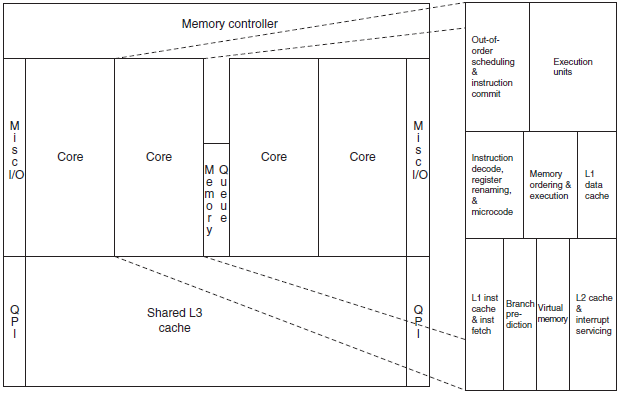
\includegraphics[scale=0.5]{mc_i7_die}
\centering
\caption{Architecture du processeur d'Intel Multicore i7 \cite{qaca17}}
\label{fig:FG_2_3}
\end{figure}

La figure \ref{fig:FG_2_3} montre un exemple d'un processeur multicœurs le processeur \textbf{Intel Core i7}, il dispose de quatre cœurs regroupés par 2. 
%
Chaque cœur a son +propre cache de niveau 1 et 2 (L1, L2) et
Ils ont un cache de niveau 3 (L3) partagé.
D’un point de vue de calcul parallèle, les différences majeures entre les processeurs multicœurs disponibles sont :
%
\subsection{Contrôleur de mémoire intégré}
%
Les fournisseurs des processeurs ont intégré un \textbf{contrôleur de mémoire} et un \textbf{bus} dans la CPU MC pour connecter la mémoire du système à pleine vitesse à ces cœurs. 
Ce connecteur (le bus qui relie les cœurs à l’IMC) est généralement partagé entre tous les cœurs du processeur. %[Coo09, AMD13]
%
\subsection{Hiérarchie de la mémoire \cite{raub13}} 
%
Vu que le système de mémoire est très lent par rapport au processeur et pour utiliser efficacement les cycles de ce dernier et réduire la pénalité de l'accès mémoire (Une puce DRAM a un temps d'accès mémoire entre 20 et 70 ns 
et un processeur à 3 GHz de fréquence, a un temps de cycle de 0.33 ns, un accès mémoire est équivalent à 60–200 cycles processeurs).
Une \textbf{hiérarchie de mémoire} est généralement utilisée, composée de plusieurs niveaux de mémoires de tailles et de vitesses d'accès différentes. La figure \ref{fig:FG_2_4} schématise cette hiérarchie avec ses différents composants et \ref{table:TBhm001} donne les valeurs associées aux métriques quantitatives mesurant ses caractéristiques, seule la mémoire principale au sommet de la hiérarchie est construite à partir de \textbf{DRAM (Dynamic Random Access Memory)}, les autres niveaux utilisent \textbf{SRAM (Static Random Access Memory)}.
L'objectif dans la hiérarchie mémoire est d'avoir un temps d'accès mémoire moyen faible en favorisant l' accès aux données à partir d'une mémoire rapide, et qui contient seulement une partie des données de la mémoire principale lente. 
Sa conception peut avoir une grande influence sur le temps d'exécution des programmes parallèles.

\begin{figure}[h]
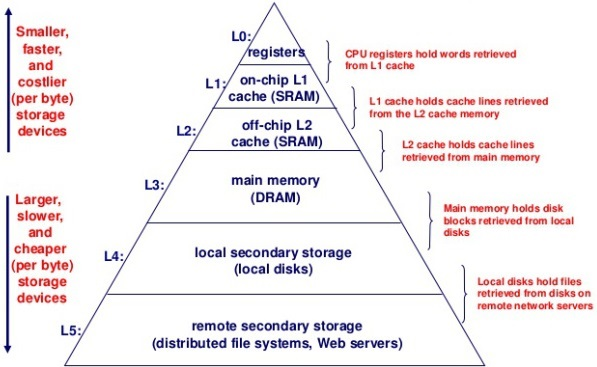
\includegraphics[scale=0.5]{memory_hierarchy01}
\centering
\caption{Hiérarchie de la mémoire}
\label{fig:FG_2_4}
\end{figure} 

\begin{table}[h!]
\centering
\begin{tabular}{| c | c | c | c | c | c | c |} 
\hline
Level                & Register    & Cache L1  & Cache L2  & Cache L3  & Memory  & Disk  \\ [0.5ex] \hline
Technology 		& Gate & SRAM & SRAM & SRAM & DRAM & Flash/Magnetic \\ [1ex]  \hline
Data 				& Word & Line (Bloc) & Line & Line & Page & File \\ [1ex]  \hline
Capacity 		& 1Kbit & 64KB & 256KB & 2-4MB & 1-16GB & 1-16TB \\ [1ex]  \hline
Latency 		& 30ps & 1ns & 3-10ns & 10-20ns & 50-100ns & 5-10ms \\ [1ex]  \hline
\end{tabular}
\caption{Caractéristiques de la hiérarchie mémoire : \cite{qaca17}} %
\label{table:TBhm001}
\end{table}
%
\subsection{Caches}
%
Tous les processeurs modernes sont équipés d'une mémoire de petite capacité (allant de quelques Ko à quelques Mo) mais très rapide (0.5-2.5 ns comparé au DRAM 50-70ns %[BK-MC-84]
) appelée \textbf{cache} SRAM qui stockent des données (une partie des données de la mémoire) sur lesquelles le processeur travaille temporairement et qui masquent la \textbf{latence d'accès} à la mémoire principale lente.
L'emplacement physique de la mémoire cache est très proche des cœurs afin de réduire les coûts de communication.

Dans une configuration typique, un CPU comprend plusieurs caches, formant une \textbf{hiérarchie de cache} %@[SZ08, OHSJ10].
Les caches peuvent être une autre ressource partagée sur les processeurs.

Le \textbf{cache de premier L1} est local pour chaque cœur de petite taille, comprise entre 8 et 128 kilo-octets, mais assez rapide. 

Le \textbf{cache du deuxième niveau L2} peut être local pour chaque cœur ou partagé entre les cœurs moins rapide que L1 et mais de taille supérieure, L1 et L2 sont partagés entre les \textbf{threads matériels}.

Le \textbf{cache de troisième niveau L3}, cependant, est partagé entre tous les cœurs du processeur de grande taille mais lent %[SZ08].

Les caches stockent les blocs de données des niveaux supérieur sous la forme de \textbf{lignes de cache = bloc} : un bloc contigu d'octets.  La taille est fixe, dépend de l'architecture, typiquement elles sont de 32 octets sur certains processeurs de l'architecture ARM [Lim07], ou 64 octets sur les processeurs x86 de l'architecture Netburst d'Intel %[Coo13b].

Grace à un \textbf{contrôleur de cache} séparé, le contrôle du cache est découplé du processeur et exécuté par ce dernier.
Pendant l'exécution du programme, 
le processeur spécifie les adresses mémoire (indépendamment de l'organisation du \textbf{système de mémoire}, sans connaître l'architecture) à lire ou à écrire comme données par les opérations de chargement/stockage. %1
il les transmet à ce système et attend que les valeurs correspondantes soient renvoyées ou écrites. %2
Après avoir reçu une requête d'accès mémoire du processeur, 
le contrôleur de cache vérifie si l'adresse mémoire spécifiée correspond à une ligne de cache qui est actuellement stockée dans le cache. %3
Si c'est le cas, une \textbf{mise en cache cache-hit} se produit et la donnée demandée est transmise au processeur à partir du cache. %4.1
Sinon un \textbf{cache manqué cache-miss} se produit et 
la ligne de cache est d'abord copiée de la mémoire dans le cache (un bloc de mémoire entier est amené dans le cache, dit un \textbf{remplacement cache})
avant que la donnée demandée ne soit délivrée au processeur. %4.2
%
Le temps de retard correspondant est appelé \textbf{pénalité du cache-miss}. 
%
Étant donné que le temps d'accès à la mémoire est significativement plus grand que le temps d'accès au cache, un cache-miss entraîne un retard de remise d'opérande au processeur.
Par conséquent, il est souhaitable de réduire autant que possible le nombre des cache-miss.
%
Le temps d'accès d'un cache dépend de sa taille, la taille du bloc-cache et sa méthode d'adressage, 
%
Toutefois, l'utilisation d'un cache plus grand entraîne un plus petit nombre de remplacements par rapport un cache plus petit, car davantage de blocs de cache peuvent être conservés dans le cache. 
%
L'utilisation de blocs plus grands réduit le nombre de blocs qui s'intègrent dans le cache lors de l'utilisation de la même taille de cache. Par conséquent, les blocs ont tendance à être remplacés plus tôt par rapport aux blocs plus petits. 

Étant donné que le cache est nettement plus petit que la mémoire principale, tous les blocs de mémoire ne peuvent pas être stockés dans le cache en même temps. 
Par conséquent, un \textbf{algorithme d'association} doit être utilisé pour définir la relation entre les blocs cache/mémoire ($BC$/$BM$) et détermine comment un bloc stocké est localisé et extrait du cache.
Pour l'association, l'accès associatif clé(tag)/valeur(contenu du $BM$) sera utilisé pour déterminer pour un bloc-mémoire les positions des blocs-cache ou il peut être stocké/sa position dans le cache pour une mise à jour ou une lecture, s'il est déjà chargé dans le cache. \cite{Hunold07}
%
\subsubsection{Méthodes de Remplacement des blocs}
%
Lorsqu'un cache-miss se produit, un nouveau bloc de mémoire doit être chargé dans le cache. Dans ce cas, il faut choisir la position dans le cache pour stocker le nouveau bloc mémoire alors il faut décharger le bloc occupant cette position.
Le bloc à remplacer est sélectionné en utilisant une méthode de remplacement.

- \textbf {Le moins récemment utilisé (Least recently used LRU)} qui remplace le bloc d'un ensemble qui n'a pas été utilisé depuis un certain temps.
le matériel doit garder une trace pour chaque bloc d'un ensemble lorsque ce dernier a été utilisé récemment et son temps d'accès correspondant doit être mise à jour à chaque utilisation.

- \textbf{Le moins fréquemment utilisé (Least frequently used LFU)} qui remplace le bloc d'un ensemble qui est le moins référencé (peu d'accès à ce bloc).
pour chaque bloc un compteur doit être maintenu par LFU qui doit être mis à jour pour chaque accès mémoire.
%
\subsubsection{Politique de modification (Write Policy)}
%
Lorsque le processeur émet un accès en écriture à un bloc de mémoire actuellement stocké dans le cache, le bloc référencé est définitivement mis à jour dans le cache, car l'accès en lecture suivant doit renvoyer la valeur la plus récente (most recent value MRV).
Quand le bloc mémoire correspondant dans la mémoire principale est-il mis à jour? La stratégie qui prend cette décision est appelé \textbf{politique d'écriture ou de modification}. Les politiques les plus utilisées sont :

- \textbf{Modification immédiate (Write-Through)}
la mise à jour de la mémoire est faite immédiatement âpres la modification du BC ce qui permet de garder la mémoire et le cache dans un état consistant. 
son inconvenant est que chaque modification cache déclenche un accès mémoire.

- \textbf {Modification retardée (Write-back)}
Une opération d'écriture d'un bloc de mémoire actuellement réside dans le cache est effectuée uniquement dans le cache; l'entrée de mémoire correspondante n'est pas mise à jour immédiatement. Ainsi, le cache peut contenir des valeurs plus récentes que la mémoire principale.
%
\subsection{Cohérence de Cache}
%
Pour les systèmes multiprocesseurs-multicœurs où chaque processeur/cœur utilise un cache local séparé, nous sommes confrontés au problème de conserver une vue cohérente des données partagées entre tous les processeurs/cœurs. 
Les données partagées stockées à des niveaux différents dans la hiérarchie de la mémoire peuvent conduire à un \textbf{problème de cohérence de cache} qui peut être défini lorsque les différents cœurs du processeur copient les mêmes informations de la mémoire/cache partagé, et que diverses copies des données seront stockées dans le cache de chaque cœur, surtout si la politique write-back est utilisée.
Par conséquent, chaque copie de données peut avoir une valeur distincte des copies des 'autres cœurs après qu'elle est traitée séparément, elle est alors appelée \textbf{copie incohérente (invalide)}. \cite{raub13}
Alors comment garder les différentes copies d'une donnée mémoire consistantes et système doit assurer l'accès à la \textbf{valeur mise a jour récemment (most recent value MRV)}?

La \textbf{cohérence des informations} entre mémoire-cache et cache-cache est un élément fondamental car elle garantit qu'un processeur/cœur a accès à la dernière valeur qui a été écrite.
Pour être cohérent, le système de mémoire doit satisfaire certaines propriétés en assurant que chaque processeur a une vue cohérente et que lui même a une \textbf{vue globale cohérente}.
Pour réaliser cet objectif, un protocole de cohérence de cache basé sur le matériel est utilisé. 
De nombreux protocoles peuvent être identifiés, y compris les protocoles de surveillance et les protocoles basés sur les répertoires.
%
\subsubsection{Protocole de surveillance}
%
Ce protocole repose sur la propriété que tous les accès mémoire sont effectués via un \textbf{support partagé de diffusion} (un bus)
de sorte que chaque contrôleur de cache puisse observer tous les accès en écriture pour effectuer des mises à jour ou des invalidations.
Ainsi, toutes les entrées peuvent être observées par les contrôleurs de cache de chaque processeur. 
Lorsque le contrôleur de cache observe une écriture dans un emplacement de mémoire actuellement détenu dans le cache local, il déclenche un mécanisme pour préserver la cohérence.
il a deux techniques :

\textbf{protocoles basés sur des mises à jour} :
Les contrôleurs de cache effectuent directement une mise à jour du cache en copiant la nouvelle valeur à partir du bus. 
Ainsi, les caches locaux contiennent toujours les valeurs écrites les plus récentes des emplacements de mémoire. 

\textbf{protocoles basés sur l'invalidation} :
Dans ce cas, le bloc de cache correspondant à un bloc de mémoire 
est invalidé de sorte que l'accès en lecture suivant doit d'abord effectuer une mise à jour à partir de la mémoire principale. \cite{Tan02}
%
\subsubsection{Protocole basé sur l'annuaire}
%
Ce protocole est une alternative au protocole de surveillance, au lieu d'utiliser un support de diffusion, il utilise un \textbf{répertoire central} pour stocker l'état des blocs de mémoire qui peuvent être conservés dans le cache. 
un contrôleur de cache peut obtenir l'état d'un bloc de mémoire par une recherche dans le répertoire. 
Ce répertoire peut être partagé ou réparti entre différents processeurs pour éviter les conflits d'accès. \cite{Culler99}

Un répertoire central est maintenu pour sauvegarder l'état de chaque bloc mémoire qui est déjà copié dans un cache. Ce répertoire peut être partagé. Le contrôleur de cache détermine l'état d'un  bloc en accédant et en consultant ce répertoire.

%=====================================================================================================================================
\section{Systèmes SMP/UMA (uniform memory access)}
%
Ils sont des multiprocesseurs à mémoire partagée via un bus commun, comportent un petit nombre de processeurs, généralement huit ou moins souvent appelés \textbf{Multiproce-sseurs symétriques (à mémoire partagée) (SMP)}.
Vue leurs conception architecturale, Les SMP et les MC ont en commun une contrainte qui limite leurs performances, la mémoire centrale partagée et l'accès à un espace d'adressage commun pour toutes les unités de traitement (soit processeurs ou cœurs). 
Toutes ces unités ont un temps d'accès égal à cette mémoire (un temps d'accès à la mémoire uniforme pour tout le monde UMA), d'où le terme \textbf{symétrique} ou l'\textbf{uniformité}. 

Un algorithme séquentiel $A_s$ parallélisé ($A_p$) pour être exécuté sur une architecture UMA peut ne pas atteindre les performances espérées préalablement (gain en rapidité et la réduction significative du temps total d'exécution $C_{max}$) pour plusieurs raisons qui peuvent être liées à 
 sa nature, 
à la méthode de la décomposition parallèle ou 
aux contraintes des architectures cibles. 
Avant d'exposer ces facteurs, nous présentons les métriques qui permettent de mesurer le gain de l'exécution parallèle sur une architecture cible par rapport son exécution séquentielle.
%
\subsection{Mesure de l'accélération (speedup $\gamma$)} 
%
\begin{définition}[Accélération d'un programme parallèle.]\textit{
%
En donnant un algorithme séquentiel $A_p$ dont le temps d'exécution séquentielle sur un processeur est $T_1$ , 
Soit $A_p$ sa version parallèle et $T_p$ son temps total d'exécution sur l'architecture parallèle cible $\mathbb{H}$.
L’\textbf{accélération} de $A_p$ représente le gain en rapidité d’exécution obtenu par son exécution sur $\mathbb{H}$ qui est égale au rapport entre le temps d’exécution du programme séquentiel et le temps d’exécution parallèle en fonction du nombre des ressources parallèles dans la plateforme (processeurs).
$$\gamma(n) = \frac{T_1}{T_p}$$
}\end{définition}
%
Si ce rapport est constant alors l’accélération est linéaire dans ce cas elle représente un parallélisme optimal (idéal). 
Mais s’il est variable sa courbe représente une accélération sub-linéaire (au dessous de la ligne $y=x$) alors ce ralentissement dû au overhead du parallélisme causé par la communication et la synchronisation.

La décomposition d’un programme parallèle influence sur ce facteur. Et puisque cette décomposition est fonction degré intrinsèque de parallélisation de l'algorithme séquen-tiel (
L’existence d'une partie purement séquentielle $T_s$ et d'une partie parallélisable $T_p$ tel que $T_1 = T_s + T_p$ avec un taux de parallélisation $\alpha_p = T_p/T_1$) . 
La \textbf{loi d'Amdahl} raffine l'expression de $gamma$ en fonction de cette décomposition et le nombre des processeurs $p$ de la plateforme parallèle, par la formule suivante \cite{raub13}:

$$ \gamma = \frac{T_1}{T_s + T_p/p} = \frac{1}{(1-\alpha_p) + \alpha_p/p}$$

On remarque que si $\lim_{p \to \infty} \gamma = 1/(1-\alpha_p)$ alors cette accélération est limitée par la partie non parallélisable de $A$. Et si $\lim_{\alpha_p \to 1} \gamma = p$ ça donne une accélération linéaire (un parallélisme optimal).

Cette mesure $\gamma$ exprime une valeur théorique qui ne prend pas en compte l'influence des opérations de la communication et la synchronisation entre les parties parallèles entre elles-mêmes ou avec la hiérarchie mémoire d'une part et l'impact de l'architecture de la plateforme parallèle (ses caractéristiques, sa topologie, ) avec son support d'exécution (runtime, ordonnanceur, mapper, ...) d'autre part. Ces deux facteurs ajoutent un overhead non négligeable aux processus de la parallélisation. 
Bien que les caches, la préextraction(pre-fetching) et les canaux de communication améliorent considérablement les performances si elles sont exploitées efficacement, pas tous les accès à la mémoire principale peuvent être éliminés et ou les communications entre les parties parallèles l'amélioration de la latence d'accès DRAM et la minimisation de l'impact de la communication/synchronisation reste une préoccupation majeure pour les performances.

Dans le contexte des architectures SMP/multicœur,
un système parallèle de $p$ unités de traitement (processeur/cœur), chaque unité supplémentaire augmente potentielle-ment le nombre total de demandes à la mémoire principale par unité de temps $t$ et le nombre des opérations communication/synchronisation $Q_M(p,t)$ et augmente ainsi la pression sur le contrôleur de mémoire et sur bus partagé en réduisant la bande passante et augmentant la latence d'accès à la DRAM $L_M(p,t)$. 

$$Q_M(p,t) \leq Q_M(p+1,t) \Rightarrow L_M(p,t) > L_M(p+1, t)$$

Pour $p_0$ suffisamment grand $L_M(p_0, t) >>$ devient important. Une fois la bande passante du contrôleur saturée, la latence des accès à la DRAM augmente et les accès mémoire deviennent rapidement un goulot d'étranglement pour les performances qui augmentent le temps des communications et par conséquent le temps total d'exécution $C_{max}$ .\\
%
\subsection{Passage à l’échelle (scalability $\zeta$)}
%
\begin{définition}[Accélération d'un programme parallèle.]\textit{
%
La scalabilité ($\zeta$) d’un programme parallèle désigne l’augmentation des performances ($\Phi$) obtenues lorsque l’on ajoute des processeurs $p$ : 
$$\zeta_p =\Delta(p) = \Phi(q+p)/\Phi(q)$$
%
}\end{définition}

La scalabilité mesure l'évolutivité qui est le degré auquel le débit de charge de travail $W$ bénéficie de la disponibilité de processeurs supplémentaires ou la faculté d'un système de maintenir un niveau de performance stable $\Phi_c$.
Il est généralement exprimé comme le quotient du débit de la charge de travail $W_p$ sur un multiprocesseur divisé par le débit sur un monoprocesseur comparable $W_1$ : $\zeta_p = W_p/W_1$.
%ref http://www.perfdynamics.com/Manifesto/USLscalability.html.
Dans leurs travaux Gunther .al propose un modèle pour quantifier la scalabilité de façon générale. Le modèle proposé USL (Universal scalabilité law) \cite{Gun17} combine les effets suivants en définissant un modèle de scalabilité unifiée dont le coefficient de scalabilité C(N) : 
%
$$ C(N) = \frac{N}{1 + \alpha (N - 1) + \beta N (N - 1)}$$
%
Les termes du dénominateur expriment les aspects suivants (les niveaux \textbf{3Cs}) :\\
- \textbf{Concurrence}: (parallelism ideal): basically, linear scaling (Computation) .\\
- \textbf{Contention}: due aux files d'attente des ressources partagées(Communication $\alpha$)\\  %overhead 
- \textbf{Cohérence}: due au retard de la mise à jour des données dans la hiérarchie mémoire (rendre les données consistantes et cohérentes) ($\beta$).

Dans le contexte des machines parallèles récentes, nous pouvons inclure les facteurs ignorés dans la loi d'Amdahl en définissant un speedup $\gamma$ étendu exprimé en fonction du parallélisme intrinsèque de la l'algorithme séquentiel (la partie parallélisable) et son overhead de la communication/synchronisation $\beta_c$ généré par son exécution parallèle sur la plateforme cible (la configuration de la plateforme c.-à-d. sa topologie, sa hiérarchie mémoire, son réseau d’interconnexion,). 
%
$$\gamma(n) = \frac{1}{(1-\alpha_p) + \alpha_p/p + \beta_c} = h( \text{algorithme\_parallèle , plateforme\_configuration})$$
%
\begin{figure}[h]
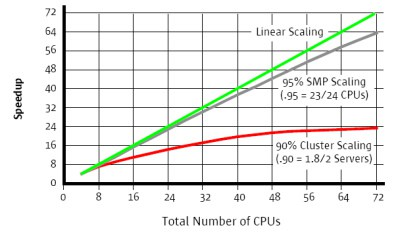
\includegraphics[scale=0.5]{scalability001}
\centering
\caption{Scalabilité linéaire, SMP et Cluster  \cite{qaca17}}
\label{fig:FG_2_5}
\end{figure}
%
La figure \ref{fig:FG_2_5} présente la scalabilité de certaines plateformes informatiques. Elle donne la mesure de l'accélération résultant du processus de la parallélisation d'une application sur une plateforme parallèle constituée de plusieurs processeurs.

L'expérimentation a démontré que les charges de travail réelles ne s'adaptent pas parfaitement à un système SMP à partir de certain seuil. 
Dans ce contexte, les principaux facteurs qui empêchent une scalabilité parfaite sont les suivants :\\
%
- \textit{La contention bus/mémoire augmente (toute la mémoire est partagée par tous les proces-seurs)}\\
- \textit{L'augmentation du coût/nombre des échecs caches (ratés)}\\
- \textit{Le cache invalidation des caches distants (lire un cache distant pour maintenir la cohérence du cache)}\\
- \textit{Augmentation du coût / nombre des instructions de synchronisation / verrouillage - déverrouillage / attente de verrous utilisés par le système d'exploitation et applications}.

Tous ces facteurs contribuent négativement à achever un niveau de scalabilité acceptable sur SMP pour des charges de travail moyennes ou importantes. 
C'est difficile dans ces conditions (SMP-mémoire partagée avec un bus d'accès unique) de préserver un niveau stable des performances en ajoutant d'autre processeurs à partir de certain seuil $p_0$ par contre toute augmentation va avoir un effet négatif sur la performance 
(Problème de scalabilité : $ \forall p > p_0, \zeta_p \leq \zeta_{p-1}$)
%======================================================================================
\section{Systèmes NUMA Non Uniform memory Access}
%
NUMA est une solution pour surmonter les problèmes de la scalabilité des architec-tures SMP \cite{lak-pan}, basée sur le principe d'une mémoire distribuée et partagée ou les processeurs accèdent à tout l'espace mémoire disponibles.
Chaque processeur est directem-ent connecté à une partie de la mémoire physique (un banc mémoire). Un exemple d'une carte mère NUMA  à quatre nœuds constitués d'un microprocesseur et d'un banc mémoire est donné dans la figure \ref{fig:FG_2_6}. La deuxième figure \ref{fig:FG_2_7} montre l'architecture typique d'une plateforme NUMA deux variantes présentées à deux nœuds et à plusieurs nœuds respectivement.
%
\begin{figure}[h]
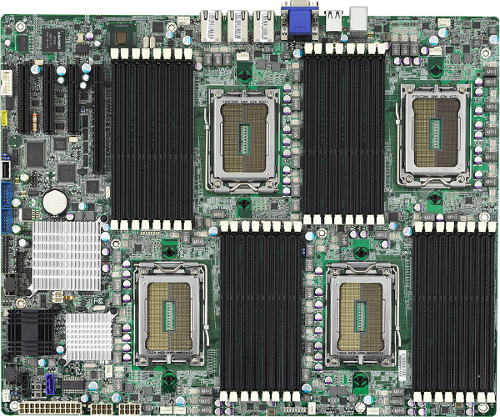
\includegraphics[scale=0.5]{mother_board_numa}
\centering
\caption{Carte mère NUMA}  % sr0c : \cite{ctan}}
\label{fig:FG_2_6}
\end{figure}
%
\begin{figure}[h]
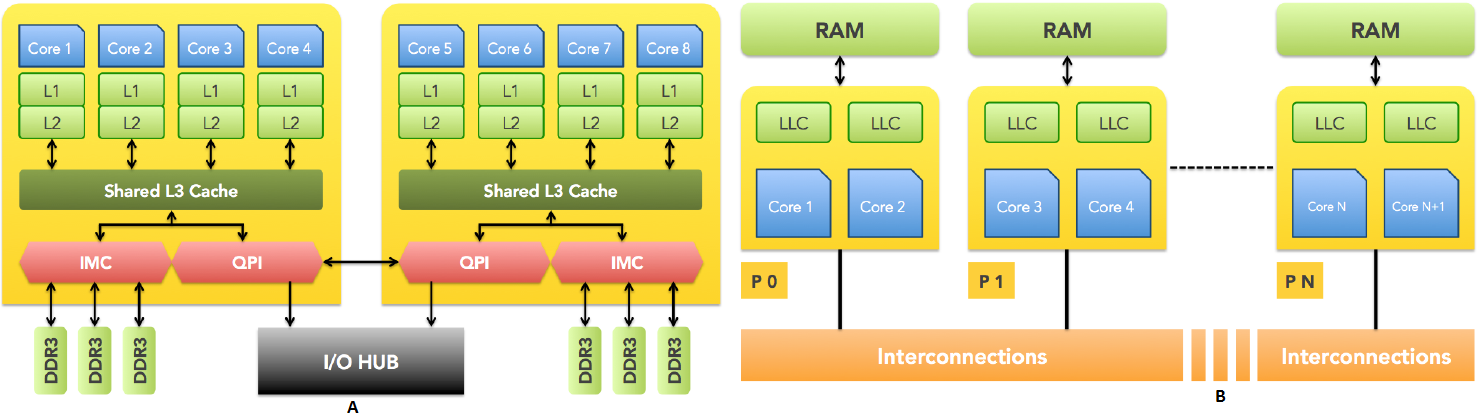
\includegraphics[scale=0.4]{numa001}
\centering
\caption{Architecture NUMA (a) Plusieurs nœuds (b) à deux nœuds }  % sr0c : /cite{ctan}}
\label{fig:FG_2_7}
\end{figure}
%
\subsection{Architecture NUMA}
Son architecture est constituée de composants suivants : 
%
\subsubsection{Nœud (Node, Socket)}
Un nœud peut être un processeur multicœurs ou un SMP constitué de plusieurs processeurs multicœurs qui se caractérise par l'uniformité de l'accès à la mémoire de tous ces composants (UMA).
%
\subsubsection{Réseaux d'interconnexion (Interconnexion network ICN)}
Un réseau de liens de communication de haut débit et de faible latence, les échanges sont établis via une connexion sur ce réseau (déterminer le chemin entre deux communicants, un routage). %deux types existe de cet ICN : 
Ce réseau est caractérisé par sa topologie déterminée par la façon de connecter les nœuds des plateformes. Deux classes de topologies existent :

A- \textbf{Topologie point-a-point (entièrement maillé)} : permet de connecter tous les nœuds en direct (un seul saut) 
Ce type de topologie dégrade les performances lors du passage à l'échelle pour un réseau moyen ou important de processeurs connectés vu que le nombre des liens requis est quadratique $O(n^2)$.

B- \textbf{Topologie spécifique avec un mécanisme de routage} : Elle peut être un arbre ou anneau ou autre avec des caractéristiques géométriques spécifiques qui permettent de déterminer la longueur du chemin pour relier deux processeurs communicants. 
Les processeurs distants sont accessibles par plus d'un saut en plusieurs étapes intermédiaires à travers d’autres processeurs. 
Le mécanisme de routage permet de déterminer le chemin menant au processeur cible à partir de la source ensuite acheminer les requêtes distantes aux processeurs cibles pour lire ou écrire une information dans sa mémoire locale à la demande du processeur source. 

Parmi les ICNs implémentés sur les plateformes NUMAs modernes, nous pouvons citer \cite{dan-mul} : \\
-a- \textbf{QPI} : QuickPath Interconnect (QPI) Intel \cite{IntelQPI09}\\
-b- \textbf{HT} : HyperTransport AMD \cite{amdHT}\\
-c- \textbf{FP}: Fireplane interconnect Sun Microsystems \cite{Char02}.
%
\subsubsection{Mémoire distribuée-partagée}
%
Le système de mémoire est hybride, une mémoire distribuée-partagée, physiquement distribuée sur les nœuds et partagée entre es cœurs de même nœud. L'espace d'adressage est global et partagé, n'importe quelle unité de calcul peut accéder à n'importe quelle adresse mémoire. Dans ce contexte, nous distinguons deux types de mémoire :\\
%
a - \textbf{Mémoire locale} : des bancs de mémoire associée à chaque processeur et directement connectés caractérisés par un accès local en écriture en lecture aux données situées dans sa mémoire locale qui est assez rapid. La figure \ref{fig:FG_2_num010} schématise les accès mémoire sur une plateforme NUMA et coût correspond en fonction des cycles processeur. Pour les accès locaux, Elle donne 38 cycles pour le cache local et 190 cycles pour la mémoire locale.\\
%
b - \textbf{Mémoire distante} : qui, du point de vue d'un CPU, est connectée à un CPU différent, caractérisée par un accès distant en écriture ou en lecture aux données situées dans une mémoire distante qui assez lent. % comme la mémoire globale est distribuée (locale à un processeur différent)
Sur la figure \ref{fig:FG_2_num010}, Pour les accès distants, Les valeurs données sont 186 cycles pour le cache distant et 310 cycles pour la mémoire distante.
%
\begin{figure}
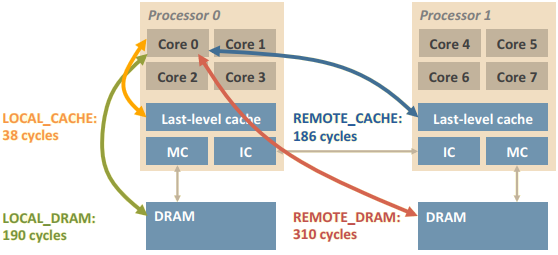
\includegraphics[scale=0.75]{num010}
\centering
\caption{Accès mémoire locaux et distants sur NUMA}
\label{fig:FG_2_num010}
\end{figure}
%
La figure \ref{fig:FG_2_num0092} présente un exemple d'un code OPENMP qui s'exécute sur NUMA en parallélisant une boucle dont les données sont deux vecteurs $A$ et $B$. Chaque itération va lire une valeur de $A$ ($A[i]$) et modifie une valeur de $B$ ($A[i]$). La parallélisation de la boucle crée un ensemble de tâches (thread) pour exécuter un nombre spécifié d'itérations. Donc chaque tâche nécessite d'accéder à la plage affectée des valeurs de $A$ et $B$ pour faire son calcul. Si les vecteurs $A$ et $B$ sont distribués sur les mémoires de la plateforme (le cas présenté par la figure), et la plage des éléments de $A$ et $B$ utilisés par la tâche $T$ est stockée dans la mémoire du nœud $N$ sur lequel $T$ s'exécute, alors les $T$ n'aura que des accès locaux. Par contre si une partie de ces éléments sont stockés sur une autre mémoire alors Certain nombre d'accès mémoire de $T$ seront distant et cela va prolonger l'exécution de $T$. Les tables \ref{table:TB_2_14520} et \ref{table:TB_2_1453} donnent le coût en cycle processeur, temps d'accès (local, voisin et voisin distant) et bande passante/latence respectivement des accès mémoire en fonction de leurs nature et emplacement. Ca donne une idée de l'impact du type d'accès sur le déroulement de l'exécution des tâches (en réduisant/augmentant le nombre de cycles processeur ou temps d'accès ou latence/BP).
%
\begin{table}[h!]
\centering
\begin{tabular}{| c | c | c | c |} 
\hline
			& CACHE		& MEMORY 	& BANDWIDTH \\ [0.5ex] \hline
LOCAL  	& 38 cycles   	& 190 cycles 	& 10.1 GB/s      \\ [0.5ex] \hline
REMOTE 	& 186 cycles 	& 310 cycles 	& 6.3 GB/s       \\ [1ex]  \hline
\end{tabular}
\caption{Coût des accès mémoire en cycles processeur et la bande passante} %
\label{table:TB_2_14520}
\end{table}
%
\begin{figure}
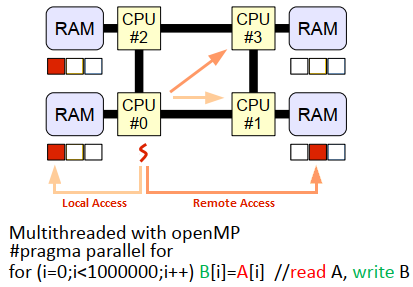
\includegraphics[scale=0.75]{num0092}
\centering
\caption{Code OPENMP parallélisant une boucle sur NUMA}
\label{fig:FG_2_num0092}
\end{figure}
%
\begin{table}[h!]
\centering
\begin{tabular}{| c | c | c | c |} 
\hline
			& LOCAL NODE		& NEIGHBOR NODE & OPPOSITE NODE\\ [0.5ex] \hline
READ  	& 83 ns   	& 98 ns  	& 117 ns\\ [0.5ex] \hline
WRITE 	& 142 ns 	& 177 ns  & 208 ns\\ [1ex]  \hline
\end{tabular}
\caption{Coût des accès mémoire mesuré en temps d'accès pour l'exemple figure \ref{fig:FG_2_num0092}} %
\label{table:TB_2_1453}
\end{table}
%
\subsection{Caractéristiques NUMA}
%
\subsubsection{Pénalité NUMA (ratio)}
%
Comparé à un accès local, l'accès distant est caractérisé par un débit faible et latence importante. En se basant sur cette réalité dans les plateformes NUMA, nous pouvons définir une métrique qui évalue l'efficacité des politiques des gestions des ressources NUMA en fonction des ces deux types d'accès. Cette métrique est appelée ratio NUMA (distance, NUMA rate, factor).
La pénalité NUMA $\alpha$ est le rapport du nombre d'accès local $A_L$ sur le nombre des accès distant $A_R$ pour le programme $P$ en court d'exécution sur une plateforme NUMA spécifique. 
Cette métrique est pour quantifier l'overhead généré par la communication entre les nœuds de la plateforme lors de cette exécution \cite{dan-mul}
%
$$
\alpha(P) = \frac{A_L}{A_R}
$$
%
\subsubsection{Distance NUMA (sauts NUMA))}
%
Les architectures à base de NUMA introduisent une notion de distance entre les composants du système (ie: nœuds, processeurs, mémoire, bus d'E/S, etc.). 
La métrique utilisée pour déterminer une distance(saut) entre les nœuds NUMA varie avec la latence et la bande passante. 
%
\subsubsection{Cohérence de Cache NUMA (ccNUMA)}
%
La mémoire globale est partagée et chaque processeur peut accéder à n'importe quel élément de données, bien qu'avec des performances réduites si l'élément de données est situé sur une banque de mémoire qui n'est pas directement connectée.
Cependant, la mémoire cache interne non partagée de chaque processeur (ou de chaque nœud pour les processeurs multi-nœuds) n'est pas accessible depuis d'autres processeurs. 
Un processeur ne sait donc pas si l'état d'un élément de données dans la mémoire principale est dans un état actuel ou si un état plus mis à jour existe dans un cache d'un autre processeur.
Ainsi, les plates-formes NUMA utilisent un mécanisme pour appliquer la cohérence du cache à travers la mémoire partagée adapté NUMA.

La plupart des systèmes NUMA sont cependant cohérents avec le cache et sont officiellement appelés plateformes ccNUMA.
Les plates-formes ccNUMA utilisent un maté-riel spécial qui permet la communication entre processeurs et les contrôleurs de cache basé généralement sur la technique du répertoire.
Pour chaque cache-manqué (lecture ou écriture), chaque processeur doit communiquer avec tous les autres processeurs afin de s'assurer que le prochain chargement de la mémoire principale est dans un état actuel et non stocké dans un autre cache.
Cette communication a un surcoût significatif.
Afin de réduire cette surcharge, nous devons éviter l'accès à la même zone de mémoire par plusieurs processeurs.
%De plus, les plateformes NUMA utilisent des protocoles de cohérence de cache spécialisés comme MOESI et MESIF qui tentent de réduire la quantité de communication entre les processeurs.
\subsubsection{Exemple}
%
IBM® Power 750 Express® \cite{IBM13} , est un système NUMA. Il est équipé de quatre cartes processeurs, et chacune contient huit cœurs et huit emplacements mémoire (considé-rées locales). Le système contient 32 cœurs et 256 Go mémoire et quatre nœuds NUMA chacun avec 8 cœurs et 64 Go mémoire locale. 
Avec le mode SMT4 (Simultaneous Multith-reading) activé, les systèmes d'exploitation voit 128 (32*4) processeurs logiques avec 32 sur chaque nœud.
Le listing suivant donne le résultat de l'exécution de la commande \textbf{numactl hardware} \cite{Linux13} sur ce système .
%
\begin{Verbatim}[formatcom=\color{blue}]
numactl hardware
available: 4 nodes (0-3)

node 0 cpus: 012 3 4 5 6 7 8 9 10 11 12 13 14 .... 25 26 27 28 29 30 31
node 0 size: 61184 MB
node 0 free: 59734 MB

node 1 cpus: 32 33 34 35 36 37 38 39 40 41 42 .... 57 58 59 60 61 62 63
node 1 size: 65280 MB
node 1 free: 63848 MB

node 2 cpus: 64 65 66 67 68 69 70 71 72 73 74 .... 89 90 91 92 93 94 95
node 2 size: 65024 MB
node 2 free: 63426 MB

node 3 cpus: 96 97 98 99 100 101 102 103 104 .... 123 124 125 126 127
node 3 size: 65024 MB
node 3 free: 63631 MB

node distances:
node 0 1 2 3
0: 10 20 20 20
1: 20 10 20 20
2: 20 20 10 20
3: 20 20 20 10
\end{Verbatim}
%
%La figure suivante \ref{fig:FG_2_ArchNUMA001} montrent un exemple d'une topologie reélle d'une plateforme NUMA extraite par l'outil HWLOC. Chaque nœud a huit cœurs et une mémoire privée de 16Go et un cache L3 de 5Mo.
%
%\begin{figure}
%\includegraphics[scale=1]{ArchNUMA001}
%\centering
%\caption{Topologie réelle d'une plateforme NUMA extraite par l'outil HWLOC}
%\label{fig:FG_2_ArchNUMA001}
%\end{figure}
%
\section{Localité des données et Politiques de Placement}
%
\subsection{Principe de la localité}
%
Le principe de localité est une propriété de programme en exécution qui établie que : 
les programmes ont tendance à \textbf{réutiliser les données et instructions} qu'ils ont utilisées récemment. 
(Un programme consacre 90\% de son temps d'exécution à seulement 10\% du code). 
Ce principe permet de prédire quelles instructions et données un programme utilisera dans un avenir proche en fonction de ses accès dans un passé récent. 
Il s'applique aux accès aux données et code. Il existe des types communs de localité de référence utilisés dans les architectures informatiques. 
La localité spatiale et temporelle peut être distinguée comme suit:
%
\subsubsection{Localité spatiale}
%
Les accès mémoire d'un programme ont une grande localisation spatiale, si le programme accède souvent à des emplacements de mémoire avec des adresses voisines à des moments successifs pendant l'exécution du programme. 
Ainsi, pour les programmes avec une grande localisation spatiale, il arrive souvent qu'après un accès à un emplacement de mémoire, un ou plusieurs emplacements de mémoire de la même ligne de cache soient également accédés peu de temps après. 
Dans de telles situations, après le chargement d'un bloc de cache, plusieurs des emplacements de mémoire suivants peuvent être chargés à partir de ce bloc de cache, évitant ainsi des erreurs de cache coûteuses. 
L'utilisation de blocs de cache comprenant plusieurs mots de mémoire repose sur l'hypothèse que la plupart des programmes présentent une localité spatiale. \cite{Ken02}
%
\subsubsection{Localité temporelle}
%
Les accès mémoire d'un programme ont une forte localisation temporelle, s'il arrive souvent que le même emplacement mémoire soit accédé plusieurs fois à des moments successifs au cours de l'exécution du programme. 
Ainsi, pour les programmes avec une haute localisation temporelle, il arrive souvent qu'après avoir chargé un bloc de cache dans le cache, les mots de mémoire du bloc de cache soient accédés plusieurs fois avant que le bloc de cache soit à nouveau remplacé. \cite{Ken02}
%En ce qui concerne la localité temporelle, la situation est la suivante: après le chargement d'un bloc de cache en raison d'un accès à la mémoire, l'emplacement de mémoire correspondant n'est accédé qu'une seule fois avant que le bloc de cache soit à nouveau remplacé. \cite{Ken02}
\subsection{Politiques de Placement}
%
L'\textbf{affinité des processus et des données} est cruciale pour gérer les problèmes causés par l'\textbf{effet NUMA}, 
ce principe consiste à préserver la proximité de threads et leurs données en en allouant aux données l'espace mémoire associées au nœud sur lequel le thread s'exécute. 
Si un thread accède à la mémoire distante, le thread peut changer son affinité CPU à exécuter localement à la mémoire ou la mémoire peut migrer vers le thread d'accès.
Ces problèmes NUMA peuvent être réduits en maintenant ou en améliorant la proximité de threads et leurs données les plus fréquemment utilisées. 
Afin d'optimiser explicitement une application pour une architecture NUMA multicœurs. 
Ce but est réalisé en sélectionnant une politique de placement appropriée qui place les threads et données en respectant leurs affinités. 
Cette politique essaye de trouver un compromis entre affectation des processeurs aux threads et l'allocation de la mémoire aux données accédées par ces threads. 
%
La figure \ref{fig:FG_2_num091} montre deux façons de distribuer les données (les éléments des deux vecteurs $A$ et $B$) des tâches qui représentent chacune un lot d'itérations sur une plage constitue d'éléments de $A$ en lecture et $B$ en écriture.
%
\begin{figure}
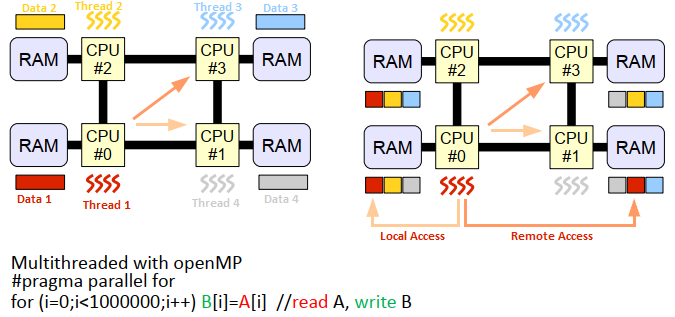
\includegraphics[scale=0.75]{num0091}
\centering
\caption{Exemples de placement des données du code OpenMP sur NUMA}
\label{fig:FG_2_num091}
\end{figure}
%
La proximité des threads à leurs données est cruciale pour la performance. 
Ceci est déterminé par les stratégies de placement du système d'exploitation et les modèles de programmation parallèle. Ces derniers souvent n'offrent aucun support explicite pour influencer le placement de la mémoire pour le programmeur.

Pour une mémoire partagée entre les processeurs à travers la plateforme avec des accès non uniformes, une distribution appropriée des données est nécessaire afin d'éviter les accès distants à la mémoire non locale. 
Les approches de la distribution des données sont :
%
\subsubsection{Round Robin}
%
En distribuant les données à tour de rôle entre les mémoires des nœuds. Elle est peu efficace et peut contribuer à amplifier l'effet NUMA en plaçant les données des threads sur des nœuds distants (aucune information n'est exploitée pour respecter l'affinité threads/données)
%
\subsubsection{Politique Affinity-on-First-Touch (AoFT)}
%
La plupart des plateformes NUMA implémentent cette première règle.
Si un thread demande un fragment de mémoire, le mappeur(qui exécute la politique de placement des données) s'assure que le fragment de mémoire est alloué à partir du segment de mémoire le plus proche à ce thread. %Elle est la plus facile à mettre en œuvre. 
La page mémoire contenant cette donnée est mappée dans le domaine local du processeur qui l'écrit en premier (c.-à-d. exécutant le thread qui a accédé à cette donnée). \cite{Mark11}
Solaris, Linux et Windows utilisent la stratégie dite de cette politique par défaut. 
Cela signifie qu'une page est placée dans la mémoire à côté du processeur à partir duquel le premier accès à la page se produit. 
Cette stratégie peut être exploitée dans une application en initialisant les données en parallèle dans le même schéma que celui auquel nous accédons pendant le calcul. 
%
\subsubsection{Politique Affinity-on-Next-Touch (AoNT)}
%
L'affinité next-touch est une autre approche pour réduire l'effet NUMA et maximi-ser l'affinité thread/données.
Lorsque l'ordonnanceur de système d'exploitation détecte qu'un processus accède à un bloc de mémoire qui ne se trouve pas dans le même nœud,
Il marque ce morceau de mémoire prêt à être déplacé.
Il essayera alors de trouver un moment approprié pour déplacer le morceau de mémoire vers le segment de mémoire approprié, qui est le plus proche du processus en cours. 
Selon Lankes et al. \cite {lak-pan} le système d'exploitation Sun / Oracle Solaris utilise la politique de distribution affinity-on-next-touch, alors que Linux n'a toujours pas cette fonctionnalité.

\textbf{Solaris} : Solaris propose l'appel système \textbf{madvise} via le MPO (optimisation du placement de la mémoire) installation, en prenant une plage d'adresses et un indicateur de modèle d'accès en tant qu'arguments. 
L'indicateur MADV ACCESS LWP indique au noyau que le prochain thread touchera la plage d'adresses spécifiée y accédera le plus fortement et pour déplacer les pages vers le noyau du thread accédant ou NUMA nœud, respectivement. 

\textbf{Linux} : Linux a un appel système supplémentaire \textbf{sys-move-pages} qui a été rendu disponible pour offrir des facilités de migration de page. 
En utilisant cette fonction, vous pouvez déplacer manuellement les pages d'un processeur à un autre. 
Mais l'application est toujours nécessaire pour savoir quel jeu de pages doit être déplacé vers quel processeur. 
En plus de cet appel système, l'outil \textbf{numactl} \cite{Linux13} peut être utilisé pour autoriser l'allocation de mémoire uniquement à partir d'un ensemble spécifié de nœuds NUMA, ou pour définir une politique d'entrelacement de mémoire. 
La mémoire sera ensuite allouée à l'aide d'une stratégie round-robin, qui peut améliorer les performances de l'application avec des modèles d'accès mémoire aléatoires. \cite{Dreb15}.

Löf et Holmgren \cite{HEN000} ont évalué une implémentation AFFINITY-ON-NEXT-TOUCH dans le mode utilisateur de sur un domaine isolé de 8 nœuds d'un Système Sun Fire 15000.
En utilisant AFFINITY-ON-NEXT-TOUCH, la performance est améliorée jusqu'à 166\%, ce qui montre ce placement de données peut avoir un impact énorme sur les performances des applications.

Goglin et Furmento \cite{GogFur09} ont implémenté AFFINITY-ON-NEXT-TOUCH pour le noyau Linux et ont comparé les performances à une implémentation de l'espace utilisateur. 
L'implémentation basée sur le noyau est environ 30\% plus rapide sur un système AMD Opteron 8347HE à quatre nœuds et affiche un surdébit significativement moins important que l'implémentation dans l'espace utilisateur pour les petites régions de mémoire. 
Cepen-dant, les auteurs concluent qu'une implémentation dans l'espace utilisateur fonctionne mieux dans les cas où des zones mémoire plus importantes utilisées par l'application doivent être migrées. 
L'implémentation mode noyau migre ces zones page par page, tandis qu'une implémentation mode utilisateur peut migrer chacune de ces zones en une seule opération avec une surcharge plus faible.
%
\subsection{Attâchement d'un Thread (Thread Binding)}
%
le système d'exploitation peut décider de déplacer un thread de son emplacement initial(\textbf{migration}). 
Cela peut entraîner une pénalité de performance, car les données du cache ainsi que la localité mémoire sont perdues. L'opération de la migration est coûteuse. 
Pour éviter cette migration, il est possible de \textbf{lier un thread} à un cœur donné ou à un sous-ensemble donné des cœurs d'un système. 
\textbf{Solaris} propose l'appel système \textbf{processor-bind()} pour lier un thread ou un ensemble de threads à un cœur spécifié. 
La fonction \textbf{sched-setaffinity()} de l'appel système \textbf{Linux} et l'appel de la fonction \textbf{SetThreadAffinityMask()} sur \textbf{Windows} s'attendent à ce qu'un masque de bits représentant les cœurs autorisés à l'exécution d'un thread spécifique. 
Une autre approche pour appliquer la liaison de thread est via des commandes spécifiques au système d'exploitation, par exemple. en utilisant la commande \textbf{taskset} ou les outils \textbf{numactl} sous \textbf{Linux} ou en appelant un programme avec \textbf{start /affinity} sur \textbf{Windows}. 
En utilisant ces outils, un processus peut être restreint à un sous-ensemble donné de cœurs de processeurs et tout thread créé par ce processus obéira à ces restrictions. 
%
\begin{table}[h!]
\centering
\begin{tabular}{| c | c | c | c | c | c | c |} 
\hline
Operating System    & AIX7.2    & FreeBSD11  & HP/UX  & Linux Arch4.1 & Solaris & Win10 \\ [0.5ex] \hline
Pin Thread             & +    & +  & +  & +  & +  & + \\ [0.5ex] \hline
Logical CPU/Node 	& +    & +  & +  & +  & +  & +  \\ [0.5ex] \hline
Mode distance        & -     & -   & -   & +   & -  & -  \\ [0.5ex] \hline
\end{tabular}
\caption{Fonctionnalités NUMA implémentées dans les systèmes d'exploitation courants} %
\label{table:TB_2_214}
\end{table}
%
La table \ref{table:TB_2_214} montre les fonctionnalités NUMA implémentées dans les systèmes d'exploitation courants.
%
%================================================================================
\newpage
\section{Conclusion}
%
Comme il n'était pas possible de continuer la course des fréquences pour les processeurs monocoeurs d'une part et les multiprocesseurs basés sur ces processeurs n'étaient pas assez puissants et soufrent de plusieurs limitations, alors multicœurs étaient une nouvelle direction pour continuer à exploiter les puissances des ordinateurs. Dans ce premier chapitre nous avons exposé les motivations de la révolution des multicœurs au début des années deux milles. En suite, nous avons présenté leurs caractéristiques et l'impact sur l'industrie logicielle (en adaptant les systèmes d'exploitation et les applications). Cette mutation a accéléré l'adoption des applications massivement parallèles par un grand nombre d'usager (développeur, scientifique,..). 
%
Les systèmes multiprocesseurs ont gagné de puissance en utilisant cette technologie, mais ils étaient pénalisés par un nombre de facteurs qui étaient intrinsèquement liés à leurs méthodes de conception classiques qui consistent à assembler les processeurs autours d'une mémoire partagée en utilisant un bus commun pour assurer l'équité de l'utilisation des ressources entre les processeurs (créant une symétrie et uniformité d'accès à la mémoire SMP/UMA). 
%
Cette utilisation intense a rapidement montré que nous ne pouvons pas continuer à concevoir les architectures parallèles avec un esprit classique (MC-SMP-UMA) vu qu'elle a exhibé des limites en donnant un niveau de performance loin de l'espéré. Un système de mémoire hiérarchique compliqué couplé à un système de communication utilisant un support partagé ont étaient les principaux facteurs responsables de la dégradation des performances (l'accès au bus partagé créant la contention de communication et limitant le passage à l'échelle, une mémoire assez lente par rapport le processeur). 
%
Le remplacement des bus par des réseaux de communication avec des mécanismes de routage d'une part et la distribution de la mémoire centrale entre les processeurs ont donné naissance à cette nouvelle conception des plateformes parallèles NUMA qui ne sont ni symétrique ni uniforme mais offrent plus d'avantages à ces applications massivement parallèles (passage à l'échelle).

Dans la partie consacrée à NUMA, nous avons décrit cette architecture en donnant ces principaux composants et comment elle contribue à surmonter le problème de passage à l'échelle des UMA. Par la suite nous avons parlé des spécificités/contraintes NUMA qui impactent grandement les politiques classiques d'ordonnancement des applications parallèles qui ne sont plus adaptées à ce contexte vu qu'elles ne sont pas concernées par la localité et le placement des données sur une mémoire distribuées et un espace d'adressage partagé. 
Alors nous avons présenté les modifications qui a été faite au système d'exploitation pour être adapté à NUMA (NUMA aware), en implémentant les politiques de placements des données standardisées ainsi que l'affinité des threads en les attachants à une unité d'exécution ou à un groupe d'unités.

Dans le chapitre suivant, nous allons parler des applications parallèles en générale et les applications parallèles décrites par un graphe de tâches en particulier.